\section{Introduction}
\label{Introduction}

The High Threshold {\v C}erenkov Counter (HTCC) is one of the major 
components of the {\tt CLAS12} spectrometer.  It will be used for 
electron identification in all experiments with electron beams.  In 
combination with the Low Threshold {\v C}erenkov Counter (LTCC), it 
will make possible the identification of charged $\pi$-mesons over 
the entire momentum range up to a maximum of 5~GeV.  An overall view 
of the {\tt CLAS12} spectrometer is given in Fig.~\ref{CLAS12}.  Part 
of the infrastructure in the Hall~B experimental area and other 
equipment are shown as well.

%%%%%%%%%%%%%%%%%%%%%%%%%%%%%%%%%%%%%%%%%%%%%%%%%%%%%%%%%%%%%%%%%%%%%%
\begin{figure}
\begin{center}
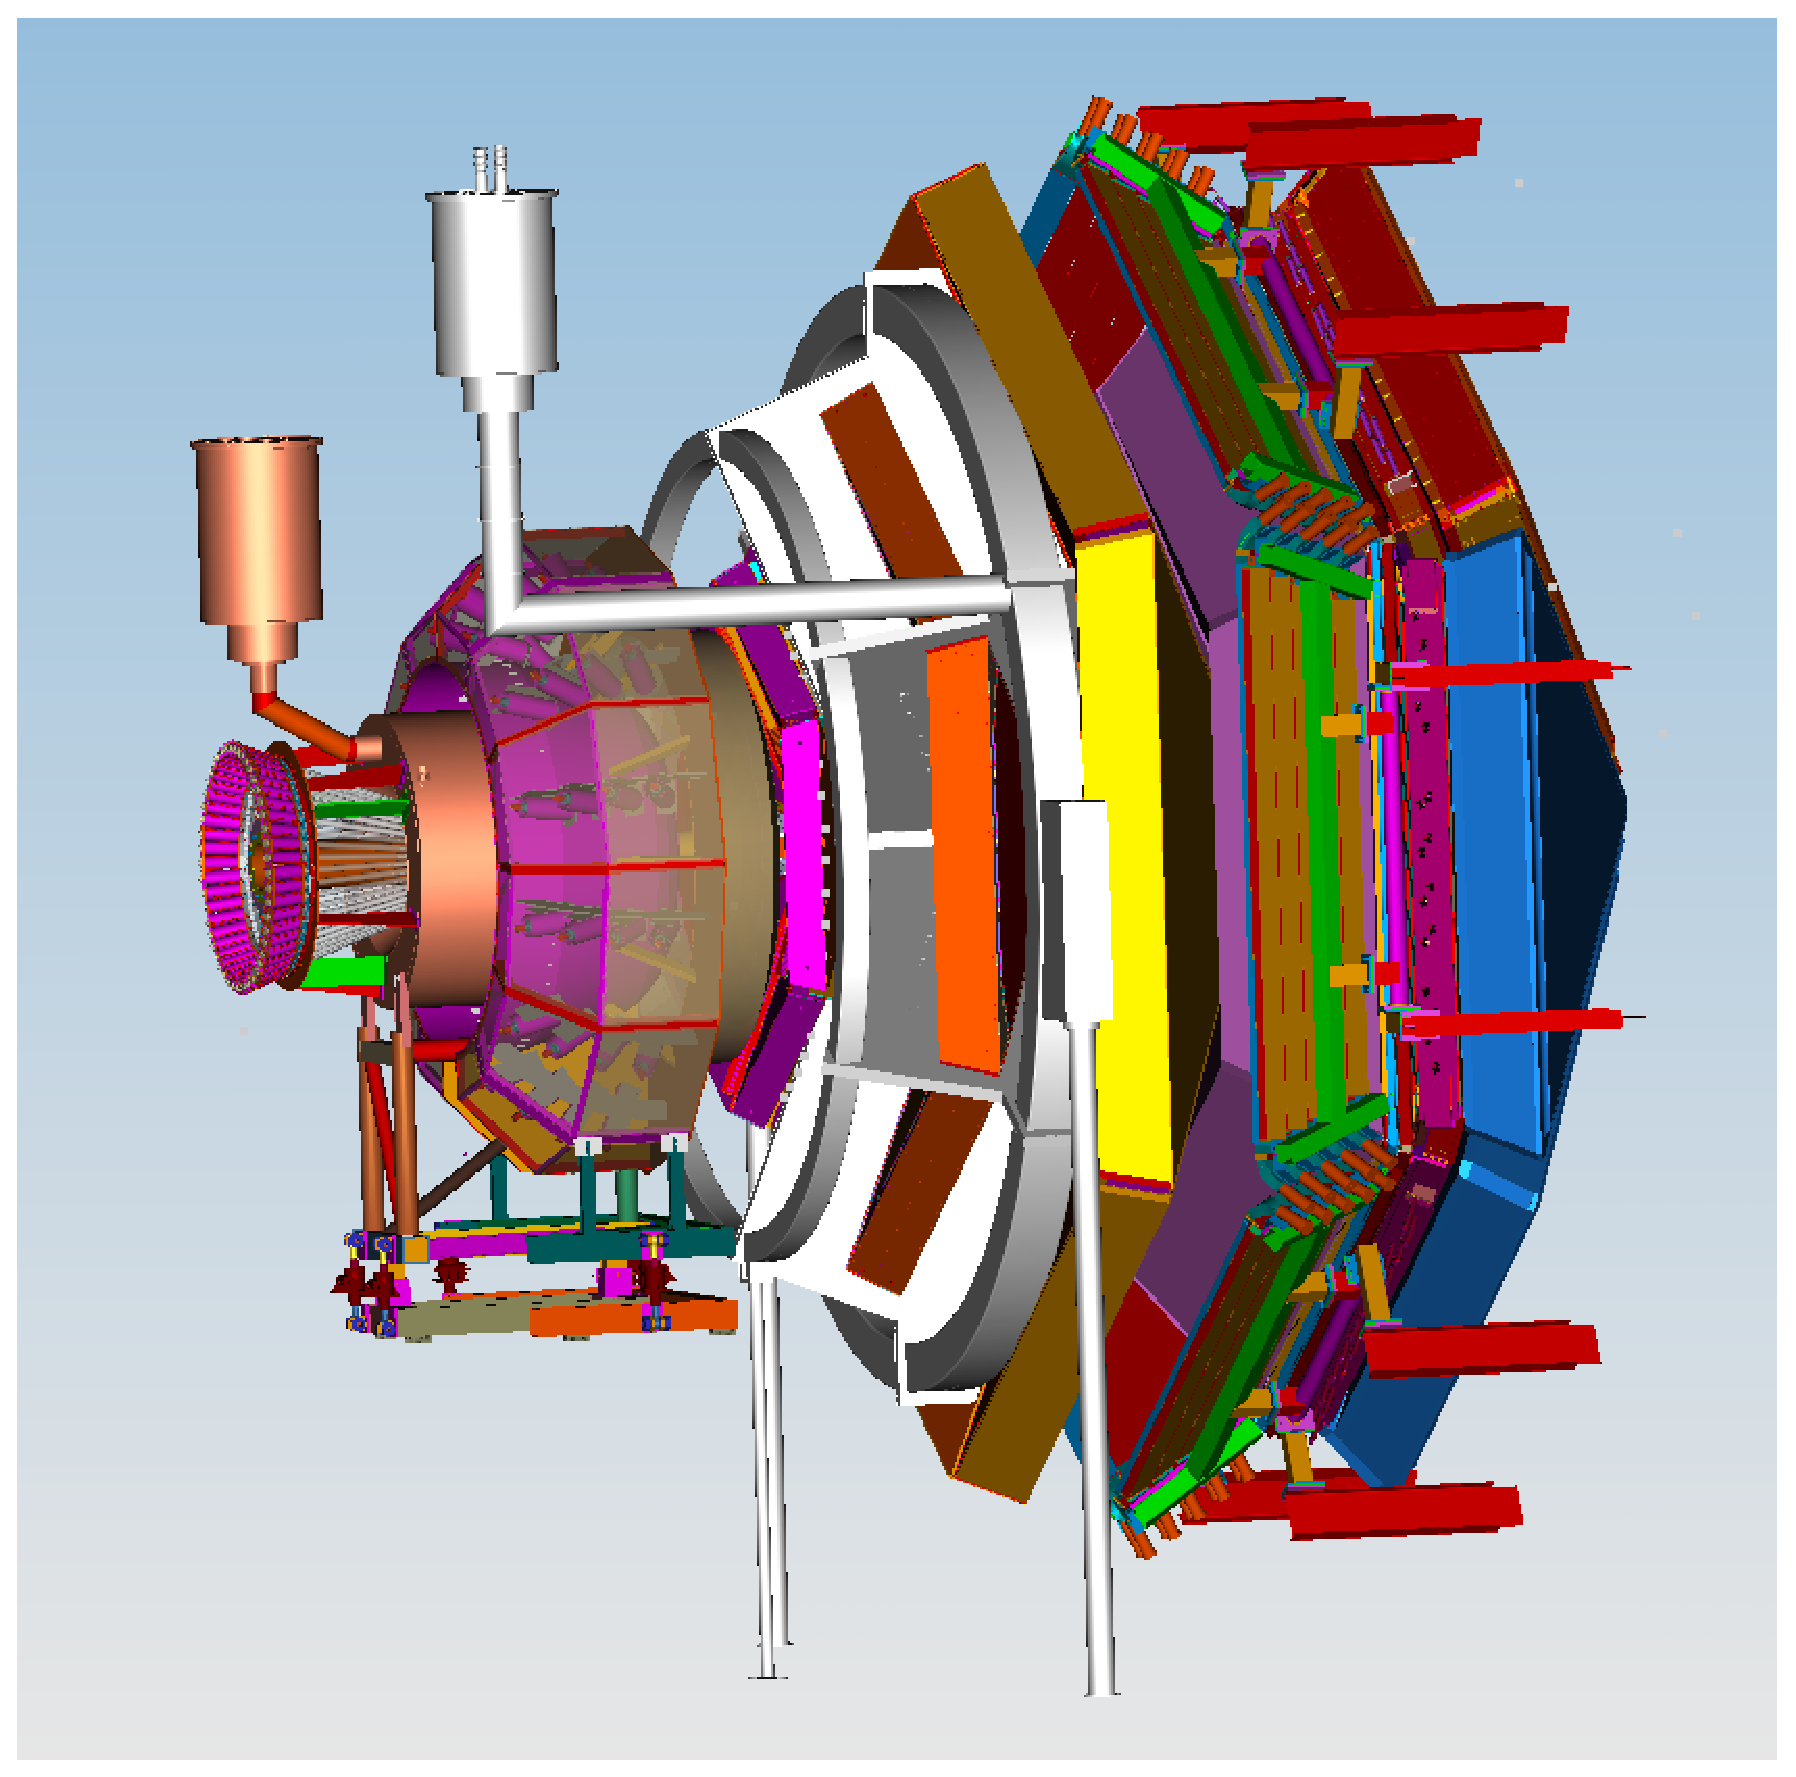
\epsfig{file=Youri/pictures/CD3_CLAS12.eps,width=10.5cm}
\caption{\small{{\tt CLAS12} spectrometer in experimental Hall~B. The
HTCC is shown mounted on the extension of Level-1 of the space frame
just downstream and outside of the solenoid.}}
\label{CLAS12}
\end{center}
\end{figure}
%%%%%%%%%%%%%%%%%%%%%%%%%%%%%%%%%%%%%%%%%%%%%%%%%%%%%%%%%%%%%%%%%%%%%%
   
The HTCC is located between the central and forward detectors of 
{\tt CLAS12}, and is mounted on a separate cart that can be moved along the 
beam direction.  The radiating gas for the HTCC is CO$_2$ at room 
temperature and pressure.  The threshold for the detection of charged 
$\pi$-mesons is 4.9~GeV.  In the entire momentum range below threshold in 
which the detection efficiency for electrons is 99.99\%, the pion rejection 
factor is greater than 300.  For 2.0~GeV pions, it is greater than 750. The 
optical configuration in the HTCC is chosen to be similar to the LTCC 
currently used in {\tt CLAS}.  However, since the detector is positioned 
upstream of the drift chambers and therefore has to be ``thin'', it was 
decided to use one reflection from a single mirror in a given module, as 
opposed to two for the LTCC.  The current design comprises 48 light 
reflection and collection modules.  The main working parameters of the 
HTCC are given in Table~\ref{htcc_parms}.  The overall performance 
requirements and the scope of the primary problems that need to be solved 
are shown in Table~\ref{htcc_reqs}.

%%%%%%%%%%%%%%%%%%%%%%%%%%%%%%%%%%%%%%%%%%%%%%%%%%%%%%%%%%%%%%%%%%%%%%
\begin{table}[htbp]
\begin{center}
\begin{tabular}{|c|c|}  \hline
Channels           & 48 (6 sectors of (2$\times$4) channels each) \\ \hline
Working Gas        & CO$_2$ at 1~atm and room temperature         \\ \hline
Mirror Type        & Ellipsoidal, 48 segments                     \\ \hline
Photomultipliers   & XP4508 (5~in, quartz face-plate)             \\ \hline
Pion Threshold     & 4.9 GeV                                      \\ \hline
Electron Threshold & 15 MeV (electrons)                           \\ \hline
Rejection Factor   & $>$300 at $p<$ 4.9 GeV                       \\ \hline
\end{tabular}
\end{center}
\caption{\small{The main working parameters for the design of the HTCC.}}
\label{htcc_parms}
\end{table}
%%%%%%%%%%%%%%%%%%%%%%%%%%%%%%%%%%%%%%%%%%%%%%%%%%%%%%%%%%%%%%%%%%%%%%

%%%%%%%%%%%%%%%%%%%%%%%%%%%%%%%%%%%%%%%%%%%%%%%%%%%%%%%%%%%%%%%%%%%%%%
\begin{table}[htbp]
\begin{center}
\begin{tabular}{|p{0.4\textwidth}|p{0.55\textwidth}|} \hline
Performance Requirement            & R\&D tasks to be addressed \\ \hline
High electron detection efficiency & Development of technology of ellipsoidal mirror construction. One reflection of {\v C}erenkov photons in most events. \\ \hline 
Run at luminosity $\geq 10^{35}$/cm$^2$s & 48 channels. Flexibility in assigning certain 
angular acceptance to a particular channel. \\ \hline
Acceptance $\Delta \phi = 2\pi$ in angular range $5^\circ \leq \theta \leq 
35^\circ$ & Designing mirrors with no support/alignment parts within the
acceptance.  No dead zones between mirror segments. \\ \hline
Total thickness $\leq$ 200~mg/cm$^2$ & Developing technology of mirror 
construction using components of low density and no residual stress. \\ \hline
Reliability & Safe maintenance and operation of the detector. PMTs and other components can be reached and 
replaced if necessary in-situ. \\ \hline
\end{tabular}
\end{center}
\caption{\small{The overall performance requirements of the HTCC and the
scope of the primary problems that need to be solved.}}
\label{htcc_reqs}
\end{table}
%%%%%%%%%%%%%%%%%%%%%%%%%%%%%%%%%%%%%%%%%%%%%%%%%%%%%%%%%%%%%%%%%%%%%%

\subsection{Optical Requirements}
\label{Optical Requirements}

The upgraded {\tt CLAS12} spectrometer incorporates several major components 
inherited from {\tt CLAS}, such as the Forward Time-of-Flight Counters, 
the Low Threshold {\v C}erenkov Counters, and the Forward Electromagnetic 
Calorimeters.  {\tt CLAS12} will be built in the same experimental area. 
This places constraints on the overall {\tt CLAS12} design, and consequently,
on all detector components, while requiring the most efficient acceptance 
coverage.

The HTCC occupies very limited space downstream of the central detector
and is mounted between the Silicon Vertex Tracker and the Region~1 drift 
chambers.  Fig.~\ref{geometry} illustrates the basic optics of the detector, 
and Fig.~\ref{3dview} shows a 3-dimensional view of the mirror and 
PMTs for one sector.  The design is such that the photons are reflected only 
once by one of the ellipsoidal mirrors and then directly impinge on the 
photocathode of a photomultiplier tube.  However, since the optical design 
must be forgiving in the sense that the light collection efficiency must be 
relatively insensitive to the target length and position, the 5-inch PMTs 
are equipped with {\it Winston} light collection cones to account for the
smearing of the photon distributions due to the influence of the magnetic 
field of the central solenoid on the particle trajectories, 

%%%%%%%%%%%%%%%%%%%%%%%%%%%%%%%%%%%%%%%%%%%%%%%%%%%%%%%%%%%%%%%%%%%%%%
\begin{figure}[ht]
\begin{center}
\epsfig{file=Youri/pictures/CD3_2D_GEO.eps,width=10cm,angle=-90}
\caption{\small{Geometry of the HTCC: an ellipsoidal mirror segment is 
obtained by revolving a corresponding ellipse about its major axis. 
Adjacent segments intersect along planes.  The resulting 4 ellipsoidal 
segments are revolved about the $y$-axis (the beam direction) through 
$\pm$15$^\circ$.  The two highlighted mirror portions are cut to accept 
polar angles from $5^\circ$ to $35^\circ$, and by the median and coil 
planes for one sector, as shown in the right figure.}}
\label{geometry}
\end{center}
\end{figure}
%%%%%%%%%%%%%%%%%%%%%%%%%%%%%%%%%%%%%%%%%%%%%%%%%%%%%%%%%%%%%%%%%%%%%%

%%%%%%%%%%%%%%%%%%%%%%%%%%%%%%%%%%%%%%%%%%%%%%%%%%%%%%%%%%%%%%%%%%%%%%
\begin{figure}
\begin{center}
\epsfig{file=Youri/pictures/CD3_3D_GEO.eps,width=10cm,angle=-90}
\caption{\small{3D-view of the mirror and the PMTs for one HTCC sector.}}
\label{3dview}
\end{center}
\end{figure}
%%%%%%%%%%%%%%%%%%%%%%%%%%%%%%%%%%%%%%%%%%%%%%%%%%%%%%%%%%%%%%%%%%%%%%

The optical properties of the mirrors, Winston cones, and PMTs are 
optimized for maximum reflection and detection of the {\v C}erenkov 
light.  Since much of the {\v C}erenkov light is in the ultraviolet (UV), 
the working surfaces of the mirrors and cones will consist of evaporated
coatings of aluminum, which has a high reflectivity from the near UV 
through the visible wavelength regions.  An evaporated magnesium fluoride 
(MgF$_2$) protective coating will be provided to prevent oxidation of the 
aluminum, while transmitting light through the required wavelength range. 
The photomultiplier tubes will be Photonis XP4508 units with a quartz 
face plate, again, to maximize efficiency in the UV range. 
 
\subsection{Physical Environment} 
\label{Physical Environment}

The HTCC is a single module detector covering all six sectors for scattering 
angles in the range $\theta = 5^\circ$ to $35^\circ$ in the entire 
$\Delta \phi = 2\pi$ range.  Since the detector is a single unit, it can be 
moved along the beam direction or removed from the beam if necessary.  It is 
located in the strong magnetic field of the superconducting solenoid of the 
central detector.  The light collection geometry of the HTCC is such that all 
48 PMTs are located in the fringe field domain at radial distances from
161.3~cm to 194.7~cm from the electron beam.  These distances are chosen to be 
maximal, while still small enough to fit in the Hall~B tunnel and space 
frame infrastructure, while allowing movement of the detector upstream for 
{\tt CLAS12} alignment and maintenance purposes.

The space occupied by the HTCC along the beam direction defines the 
intensity of the {\v C}erenkov photons expected at a given pressure of the 
working gas.  The design of {\tt CLAS12} specifies that the entrance window 
of the {\v C}erenkov counter is located $\sim$0.5~in downstream of the SVT 
of the central detector, and the exit window is 10~cm upstream of the Region~1 
drift chambers.  That leaves the distance that the scattered electrons travel 
in the CO$_2$ radiator of $\sim$131~cm at $\theta = 5^\circ$ and $\sim$181~cm 
at $\theta = 35^\circ$.  The geometry of the HTCC is optimized to keep the
differences in path lengths minimal.  The distribution of magnetic fringe 
fields was taken into consideration in locating the PMTs.  The optics and
estimated signal strength are discussed below.

The intrinsic angular and momentum resolutions of {\tt CLAS12}, along with 
its capability of running at high luminosities, puts serious constraints on 
both the thicknesses and materials that can be used in the HTCC mirror 
construction.  These limitations on materials and estimates of required and 
achievable mirror thicknesses are given in Section~\ref{Mirror}.
 
Another constraint comes from the acceptance specifications for the
Region~1, 2, and 3 (R1, R2, and R3, respectively) drift chambers, which are 
located downstream of the HTCC.  The polar angle acceptance for the drift 
chambers, $\theta = 5^\circ $ to $40^\circ$, is greater than for the HTCC. 
The support structure for the elliptical mirrors has to be located in the 
relatively narrow {\it shadow} region of the coil planes of the {\tt CLAS12} 
torus magnet, and the mirror substrate support built of as light materials 
as possible.
 
\subsection{Overall Design}
\label{Overall design}

The overall approach to working out the HTCC design is a two-fold task,
first to outline the general demands on the HTCC performance and then to 
define the ranges for critical parameters of the major components such 
as the ellipsoidal mirrors.

The main requirements are:

\begin{itemize}
\item High electron detection efficiency, low background;
\item Capability of running at a luminosity of 
$1 \times 10^{35}$~cm$^{-2}$s$^{-1}$;
\item Angular acceptance $5^\circ \leq \theta \leq 35^\circ$ and
$\Delta \phi \approx 2 \pi$;
\item Lightweight -- as little material as possible within the acceptance to 
meet the expected angular and momentum resolutions of {\tt CLAS12} ($\delta 
\theta \leq 1.5$~mrad, $\delta \phi \leq 5$~mrad, and $\Delta p/p \leq 1\%$).
\end{itemize}

%%%%%%%%%%%%%%%%%%%%%%%%%%%%%%%%%%%%%%%%%%%%%%%%%%%%%%%%%%%%%%%%%%%%%%
\begin{figure}
\begin{center}
\epsfig{file=Youri/pictures/CD3_FIG2_3_1.eps,width=7cm,angle=-90}
\caption{\small{A view of the front face of the HTCC showing the 
entrance window in red.}}
\label{back}
\end{center}
\end{figure} 
%%%%%%%%%%%%%%%%%%%%%%%%%%%%%%%%%%%%%%%%%%%%%%%%%%%%%%%%%%%%%%%%%%%%%%

A front view of the HTCC is shown in Fig.~\ref{back}.  Some specific 
features of the HTCC design include:

\begin{itemize}
\item Thin entry and exit windows of black Kapton or Tedlar film\\ 
($\sim$3.5~mg/cm$^2$ and $\sim$11~mg/cm$^2$, respectively);
\item Ultra-thin, self-supporting mirror structure;
\item Capability of working with different types of Tungsten M{\o}ller 
shields. 
\end{itemize}

The total radiation length of the detector is $\sim$1.7\%, including 
contributions of the CO$_2$ radiator gas ($\sim$0.9\%), and of the mirror 
($<0.8$\%). Since the number of photons per event is proportional to the 
total radiation length of the radiator, the only way to decrease the 
thickness of the detector without compromising its performance is to use 
thinner mirror backing.  Figs.~\ref{resolution}a, b, and c illustrate the 
changes in the {\tt CLAS12} resolution for different mirror thicknesses: 
standard ($\sim$200~mg/cm$^2$) and reduced to $\sim$100~mg/cm$^2$.  The 
results show relatively small improvements in momentum, angular, and spatial 
resolutions for thinner mirrors, indicating that the influence of the mirror 
thickness is small or comparable with contributions of other {\tt CLAS12} 
detector components.

%%%%%%%%%%%%%%%%%%%%%%%%%%%%%%%%%%%%%%%%%%%%%%%%%%%%%%%%%%%%%%%%%%%%%%
\begin{figure}
\begin{center}
\epsfig{file=Youri/pictures/FIG2_3_2a.eps,width=6.5cm,angle=-90}
\vspace{0.5in}
\epsfig{file=Youri/pictures/FIG2_3_2b.eps,width=6.5cm,angle=-90}
\vspace{0.5in}
\epsfig{file=Youri/pictures/FIG2_3_2c.eps,width=6.5cm,angle=-90}
\vspace{0.5in}
\caption{\small{Momentum, angular, and spatial resolution of {\tt CLAS12} 
for pions.}}
\label{resolution}
\end{center}
\end{figure} 
%%%%%%%%%%%%%%%%%%%%%%%%%%%%%%%%%%%%%%%%%%%%%%%%%%%%%%%%%%%%%%%%%%%%%%

\section{Optical Design and Construction}
\label{Details}

The most challenging aspect of the HTCC is the construction of the
elliptical mirrors.  In addition to being very lightweight and 
self-supporting, there must not be shadowing among adjacent mirrors or gaps 
between them. This problem has been worked out as follows: each mirror 
surface is an ellipsoid of rotation, so the line of intersection of adjacent  
mirror surfaces is curved.  Two coplanar ellipses, each revolved about its 
major axis, give two ellipsoids of rotation, (1) and (2), represented by the
following equations:
 
\begin{eqnarray}
\label{elips}
\frac{x^2+(y-y_1)^2}{a_1^2} &+& \frac{(z-z_1)^2}{b_1^2} = 1  \nonumber\\
\hspace{1in}\\
\frac{x^2+(y \cdot \cos \theta-z \cdot \sin \theta)^2}{a_2^2} &+& 
\frac{(y \cdot \sin \theta-z \cdot \cos \theta)^2}{b_2^2} = 1. \nonumber  
\end{eqnarray}

\noindent
In the above, $(0,y_1,z_1)$ are the coordinates of the center of the ellipse 
(1), $a_1, a_2$, and $b_1, b_2$, respectively, are the minor and major radii 
of the ellipses, and $\theta$ is the angle between the major axis $b_2$ and 
the $z$-axis in the $y-z$-plane.  Considering the system in the $x = c < a_1$  
plane, we get (assuming $a_1 < a_2$): 

\begin{eqnarray}
\label{elips_var}
\frac{(y-y_1)^2}{a_1^2} &+& \frac{(z-z_1)^2}{b_1^2} = c_1^2 \nonumber \\
\hspace{1in}\\
\frac{(y \cdot \cos \theta-z \cdot \sin \theta)^2}{a_2^2} &+& 
\frac{(y \cdot \sin \theta-z \cdot \cos \theta)^2}{b_2^2} = c_2^2. \nonumber  
\end{eqnarray} 
 
By excluding one variable from eq.(\ref{elips_var}), we arrive at a general 
quartic equation:

\begin{equation}
p_0z^4 + p_1 z^3 + p_2 z^2 + p_1 z + p_4=0, \nonumber \\
\end{equation} 

\noindent
which always can be solved, and in the case of the HTCC geometry, has 
two roots (see Fig.~\ref{figelips}). So, from eq.(\ref{elips_var}),  
we obtain two roots $P_1^{(c)}(y_1,z_1)$ and $P_2^{(c)}(y_2,z_2)$ 
in the plane $x = c$; they also satisfy eq.(\ref{elips}) at $x = c$: 
$P_1^{(c)}(c,y_1,z_1)$ and $P_2^{(c)}(c,y_2,z_2)$ are the roots of 
eq.(\ref{elips}).  Two other roots of eq.(\ref{elips}) can be found at 
$x=0$ (the $y-z$-plane): $P_3(0,y_1,z_1)$ and $P_4(0,y_2,z_2)$.  Three out 
of any four roots define a plane.  It can be shown that the remaining 
root belongs to the same plane as well.  Since we arbitrarily used $x = c$,  
all points of intersection (intersection curve) of the two ellipsoids belong
to the same plane.  This allows us to build mutually self-supporting
ellipsoidal mirrors in which there are no gaps or shadowing of one mirror by 
the next.  As a result, the cutting of the segments along the perimeter and
the final assembly become relatively simple. Moreover, there will be no 
shadowing of one mirror by another, and no ``dead'' zones for any electrons 
from the target within the acceptance.  This also eliminates the need of 
having a support structure for any single mirror segment, and consequently 
makes it possible to construct the most efficient and lightweight mirror. 

%%%%%%%%%%%%%%%%%%%%%%%%%%%%%%%%%%%%%%%%%%%%%%%%%%%%%%%%%%%%%%%%%%%%%%
\begin{figure}
\begin{center}
\epsfig{file=Youri/pictures/CD_2_FIG2_4_1.eps,width=10cm,angle=-90}
\caption{\small{Ellipses of adjacent mirrors intersecting in two points.}}
\label{figelips}
\end{center}
\end{figure} 
\begin{figure}
\begin{center}
\epsfig{file=Youri/pictures/CD3_PLANES.eps,width=10cm,angle=-90}
\caption{\small{Planes of intersection of adjacent mirror segments.}}
\label{planes}
\end{center}
\end{figure} 
%%%%%%%%%%%%%%%%%%%%%%%%%%%%%%%%%%%%%%%%%%%%%%%%%%%%%%%%%%%%%%%%%%%%%%

Fig.~\ref{planes} shows four intersecting mirrors forming half of the mirror  
array for one sector.  The coordinates of the points defining the planes of 
intersection between segments were used in the corresponding Monte Carlo 
simulations.  Fig.~\ref{mirror} illustrates the concept of the compound 
elliptical mirror assembly.  The approximate dimensions of segment \#4 
are given in inches.

%%%%%%%%%%%%%%%%%%%%%%%%%%%%%%%%%%%%%%%%%%%%%%%%%%%%%%%%%%%%%%%%%%%%%%
\begin{figure}
\begin{center}
\epsfig{file=Youri/pictures/CD3_SEGM_CUT.eps,width=8cm,angle=-90}
\caption{\small{Elliptical mirror segments cut along the planes of 
intersection.  A set of four segments cover half of the acceptance of one 
sector.  An identical set covers the other half of the acceptance.}}
\label{mirror}
\end{center}
\end{figure} 
%%%%%%%%%%%%%%%%%%%%%%%%%%%%%%%%%%%%%%%%%%%%%%%%%%%%%%%%%%%%%%%%%%%%%%

The tolerances for construction are critical for HTCC performance. 
The typical tolerances for cutting the substrates are of order 0.001~in 
and have been achieved in prototyping.  So, the expected average
deviation from the nominal geometry would be mostly due to the accuracy that 
can be achieved at the assembly stage.  It is anticipated to keep the assembly 
tolerance within $\pm$0.010~in for one mirror segment.  Parallel shifts 
will not affect the light collection because of the large overall acceptance,
whereas unwanted rotation of a segment during assembly might require some 
adjustment of the PMT positions, which would be unacceptable.  At the given 
average half width of the segments, $\sim$5~in (see Fig.~\ref{mirror}), the
angular equivalent of $\pm$0.01~in is $\sim$2~mrad or less.  This is the 
worst possible case since all segments except \#1 are of length greater than 
5.60~in.  The average distance between the mirrors and the corresponding PMTs 
is $\sim$80.5~in. Therefore, the shift of the image in the focal plane of 
the PMTs is less then 0.15~in ($\sim$3.8~mm). This estimate will be
examined in R\&D. 

\subsection{Mirror Prototyping}
\label{Mirror}
 
All of the main features of the HTCC and the properties of its components 
will be examined and checked by prototyping and testing of the key elements. 
In this section we present results on the prototyping of one mirror segment 
obtained in FY06, and describe current R\&D efforts on building a mirror 
consisting of 3 mirror segments.  The main R\&D goal is to find ways of 
building an elliptical mirror of:

\begin{itemize}
\item 200 mg/cm$^2$ total thickness;
\item minimal residual stress (no adjustment in-situ);
\item highest possible specular reflectivity of working surface;
\item reasonable cost.
\end{itemize}

A mirror substrate consists of a thermally shaped plain Mylar film of 
thickness 0.005~in, laminated to an ellipsoidal substrate made of rigid 
Polymethacrylimide polymer foam Rohacell HF31 ($\rho \approx 31$~mg/cm$^3$). 
In the entire construction procedure, the working surface of the Mylar film 
stays untouched. The aluminum reflector and optical coating of magnesium 
fluoride (MgF$_2$) will be vacuum deposited onto the mylar surface after 
the substrate and mylar are joined as a completed unit. A set of molding 
tools is used for the shaping of the Mylar film into the ellipsoidal shape 
that mates precisely with the Rohacell substrate to avoid residual stresses.  
One of the mold fixtures attached to the bottom-plate of the vacuum chamber 
is shown in Fig.~\ref{mold}.  The top surface of the mold is cut to the 
precise shape of the specified ellipsoid of rotation by computer-controlled 
milling using a ball-end mill. The thickness of the film is taken into 
account.  The top of the mold is then polished to remove scalloping left 
after milling.  The Mylar film is shaped by this surface, so the finish 
has to be smooth enough to avoid a {\it'' telegraph wire''} effect, although 
the surface does not have to be of mirror quality.  
 
%%%%%%%%%%%%%%%%%%%%%%%%%%%%%%%%%%%%%%%%%%%%%%%%%%%%%%%%%%%%%%%%%%%%%%
\begin{figure}
\begin{center}
\epsfig{file=Youri/pictures/CD_2_MOLD.eps,width=10cm,angle=-90}
\caption{\small{The mold installed on the bottom-plate.}}
\label{mold}
\end{center}
\end{figure} 
%%%%%%%%%%%%%%%%%%%%%%%%%%%%%%%%%%%%%%%%%%%%%%%%%%%%%%%%%%%%%%%%%%%%%%

For better control of the Mylar film edges and to minimize effects of 
thermal contraction, a thin aluminum support guard is installed surrounding 
the mold, as shown in Fig.~\ref{support1}.  There is a small gap of 1/8-in 
width left between the support and mold.  The support has a profile (shown 
in red) parallel to the edge of the ellipsoidal surface of the mold.  The gap 
is so small that the edge of the shaped Mylar film is defined not by the
mold, but by the support.  This results in a better alignment of the film 
with the foam substrate while gluing.

%%%%%%%%%%%%%%%%%%%%%%%%%%%%%%%%%%%%%%%%%%%%%%%%%%%%%%%%%%%%%%%%%%%%%%
\begin{figure}
\begin{center}
\epsfig{file=Youri/pictures/CD_2_SUPPORT.eps,width=10cm,angle=-90}
\caption{\small{The support installed around the mold.}}
\label{support1}
\end{center}
\end{figure}  
%%%%%%%%%%%%%%%%%%%%%%%%%%%%%%%%%%%%%%%%%%%%%%%%%%%%%%%%%%%%%%%%%%%%%%

In Fig.~\ref{vacuum} the wall of the vacuum chamber (molding box) attached 
to the bottom plate is shown.  There are high-temperature-rated vacuum 
o-rings installed both on the top and bottom of the wall.
 
%%%%%%%%%%%%%%%%%%%%%%%%%%%%%%%%%%%%%%%%%%%%%%%%%%%%%%%%%%%%%%%%%%%%%%
\begin{figure}
\begin{center}
\epsfig{file=Youri/pictures/CD_2_WALL.eps,width=7cm,angle=-90}
\caption{\small{The vacuum chamber with the mold.}}
\label{vacuum}
\end{center}
\end{figure}  
%%%%%%%%%%%%%%%%%%%%%%%%%%%%%%%%%%%%%%%%%%%%%%%%%%%%%%%%%%%%%%%%%%%%%%

The profile of the top of the wall is cylindrical, such that there is an 
approximately constant clearance of $\sim$1/4~in between this surface and 
the ellipsoidal surface of the mold.  The inside gap between the wall and 
support is quite wide.  It has to be wide enough for the Mylar film to 
form concave channels under applied pressure.  These channels are formed all 
the way around the support and are necessary for tension relief when the  
chamber is being cooled down and then depressurized.

%%%%%%%%%%%%%%%%%%%%%%%%%%%%%%%%%%%%%%%%%%%%%%%%%%%%%%%%%%%%%%%%%%%%%%
\begin{figure}
\begin{center}
\epsfig{file=Youri/pictures/CD_2_MYLAR.eps,width=10cm,angle=-90}
\caption{\small{The vacuum chamber with the mold and the pre-cut Mylar film.}}
\label{Mylar}
\end{center}
\end{figure} 
%%%%%%%%%%%%%%%%%%%%%%%%%%%%%%%%%%%%%%%%%%%%%%%%%%%%%%%%%%%%%%%%%%%%%%

A portion of Mylar film is placed on top of the vacuum chamber, as shown 
(in transparent yellow) in Fig.~\ref{Mylar}. The top surface of the 
Mylar remains untouched during cutting and installation of the film. 
A flange is placed on the top of the Mylar and tightened down to the wall.
Then the air in the chamber is pumped out so that the Mylar is 
deflected under atmospheric pressure, as in Fig.~\ref{Mylar_var}.

%%%%%%%%%%%%%%%%%%%%%%%%%%%%%%%%%%%%%%%%%%%%%%%%%%%%%%%%%%%%%%%%%%%%%%
\begin{figure}
\begin{center}
\epsfig{file=Youri/pictures/CD_2_FLANGE.eps,width=10cm,angle=-90}
\caption{\small{The vacuum chamber with the mold and the Mylar film.}}
\label{Mylar_var}
\end{center}
\end{figure} 
%%%%%%%%%%%%%%%%%%%%%%%%%%%%%%%%%%%%%%%%%%%%%%%%%%%%%%%%%%%%%%%%%%%%%%

At this point, while still at room temperature, the Mylar is touching 
the mold, and the area of contact between them is about 60-70\% of maximum. 
To provide a 100\% contact, the vacuum chamber is heated in an oven to
a temperature of 170$^\circ$C. During the heating process, which takes about 
4~hours, the chamber remains connected to a vacuum pump located outside the 
oven.  To increase the deflection of the unsupported portion of Mylar film 
(along the wall), additional pressure is applied to the film.  This is done 
by covering the vacuum chamber with a lid installed on the top of the flange, 
as shown in Fig.~\ref{Mylar_pres}.  The volume under the lid is then 
pressurized with dry nitrogen.

%%%%%%%%%%%%%%%%%%%%%%%%%%%%%%%%%%%%%%%%%%%%%%%%%%%%%%%%%%%%%%%%%%%%%%
\begin{figure}
\begin{center}
\epsfig{file=Youri/pictures/CD_2_LID.eps,width=7cm,angle=-90}
\caption{\small{Vacuum chamber equipped with lid allowing molding of Mylar 
film at higher pressures.}}
\label{Mylar_pres}
\end{center}
\end{figure} 
%%%%%%%%%%%%%%%%%%%%%%%%%%%%%%%%%%%%%%%%%%%%%%%%%%%%%%%%%%%%%%%%%%%%%%

The maximal differential pressure applied to the Mylar can be as high 
as 3~kg/cm$^2$.  Tested stable results were obtained at differential 
pressures in the range from 2.0 to 2.55~kg/cm$^2$, depending on the
temperature.  The cooling of the chamber back to room temperature is the 
last step in the thermal shaping.  The working differential pressure, once 
reached, is monitored and kept constant during the entire cooling cycle. 
After completion, the differential pressure is brought back to atmosphere 
and the lid is removed.  A frame, shown in Fig.~\ref{glue}, is glued onto 
the already shaped Mylar film. The bottom surface of the frame has the 
required ellipsoidal shape.  On the top there is a groove cut for a vacuum 
o-ring.  In the figure, several installed studs are shown in red. 
Fig.~\ref{glue_var} illustrates the gluing of the frame onto the pressurized 
thermally shaped Mylar.  The largest portion of the Mylar, even while 
pressurized, is stress free.  That portion of the surface that is in full 
contact with the mold, is leaning on it, and therefore no stresses are 
involved here. Only the unsupported deflected portion of Mylar that is out 
of the gluing frame is under stress.  After the glue is polymerized, a flat 
Plexiglas lid is attached to the frame, and the vacuum chamber is released. 
The deflected portion of Mylar provides stress relief.  The Mylar film, 
shaped at no residual stress, together with the frame and lid, is cut out as a 
single unit for future use. 

%%%%%%%%%%%%%%%%%%%%%%%%%%%%%%%%%%%%%%%%%%%%%%%%%%%%%%%%%%%%%%%%%%%%%%
\begin{figure}
\begin{center}
\epsfig{file=Youri/pictures/CD_2_FRAME.eps,width=10cm,angle=-90}
\caption{\small{The HTCC gluing frame.}}
\label{glue}
\end{center}
\end{figure} 
%%%%%%%%%%%%%%%%%%%%%%%%%%%%%%%%%%%%%%%%%%%%%%%%%%%%%%%%%%%%%%%%%%%%%%

%%%%%%%%%%%%%%%%%%%%%%%%%%%%%%%%%%%%%%%%%%%%%%%%%%%%%%%%%%%%%%%%%%%%%%
\begin{figure}
\begin{center}
\epsfig{file=Youri/pictures/CD_2_FRAME_LID.eps,width=10cm,angle=-90}
\caption{\small{Gluing frame with Plexiglas lid on the top and Mylar 
attached to the bottom.}}
\label{glufr}
\end{center}
\end{figure}
%%%%%%%%%%%%%%%%%%%%%%%%%%%%%%%%%%%%%%%%%%%%%%%%%%%%%%%%%%%%%%%%%%%%%%

%%%%%%%%%%%%%%%%%%%%%%%%%%%%%%%%%%%%%%%%%%%%%%%%%%%%%%%%%%%%%%%%%%%%%%
\begin{figure}
\begin{center}
\epsfig{file=Youri/pictures/CD_2_FRAME_GLUED.eps,width=10cm,angle=-90}
\caption{\small{The frame glued onto the thermally shaped Mylar film leaves 
the film stress free after the chamber is depressurized.}}
\label{glue_var}
\end{center} 
\end{figure}
%%%%%%%%%%%%%%%%%%%%%%%%%%%%%%%%%%%%%%%%%%%%%%%%%%%%%%%%%%%%%%%%%%%%%%

The other important component of the mirror is the mechanical support
substrate, which is made of rigid foam.  A sheet of polymer foam is sanded 
down, under its own weight, until it provides a flat base.  The top of the 
flat sheet is cut by CNC milling to the concave ellipsoidal shape, which 
mates to the back surface of the Mylar mirror substrate, as seen in 
Fig.~\ref{flatface}.  The length and width are appropriate for gluing the 
frame and mold.

%%%%%%%%%%%%%%%%%%%%%%%%%%%%%%%%%%%%%%%%%%%%%%%%%%%%%%%%%%%%%%%%%%%%%%
\begin{figure}
\begin{center}
\epsfig{file=Youri/pictures/FIG2_5_9.eps,width=10cm,angle=-90}
\caption{\small{The substrate: flat face down, cylindrical top.}}
\label{flatface}
\end{center} 
\end{figure}
%%%%%%%%%%%%%%%%%%%%%%%%%%%%%%%%%%%%%%%%%%%%%%%%%%%%%%%%%%%%%%%%%%%%%%

In order to process the front (working) surface, the substrate is mounted 
on an auxiliary table and glued to it along the edges at several locations, 
as shown in Fig.~\ref{auxiliar}.  The top of the table and back of the 
substrate have precisely the same ellipsoidal shape, thus providing the 
required rigidity for further processing.

%%%%%%%%%%%%%%%%%%%%%%%%%%%%%%%%%%%%%%%%%%%%%%%%%%%%%%%%%%%%%%%%%%%%%%
\begin{figure}
\begin{center}
\epsfig{file=Youri/pictures/FIG2_5_10.eps,width=8cm,angle=-90}
\caption{\small{The substrate mounted on the auxiliary table.}}
\label{auxiliar}
\end{center} 
\end{figure}
%%%%%%%%%%%%%%%%%%%%%%%%%%%%%%%%%%%%%%%%%%%%%%%%%%%%%%%%%%%%%%%%%%%%%%

Fig.~\ref{computer} shows the cutting of the working surface to the shape 
of an ellipsoid.  The ellipsoid parameters were defined by taking into
account the thickness of the anticipated glue joint and of the thermally 
shaped Mylar film.  The process was optimized to achieve a surface finish 
on the foam smooth enough so that no polishing would be necessary. Due to 
the properties of foam structure, there were no scallops observed after 
milling.  In Fig.~\ref{prototype} sample pieces of the thermally shaped 
Mylar films are shown, along with the mold used in shaping them, and the 
completely processed foam substrate mounted on the auxiliary table.

%%%%%%%%%%%%%%%%%%%%%%%%%%%%%%%%%%%%%%%%%%%%%%%%%%%%%%%%%%%%%%%%%%%%%%
\begin{figure}
\begin{center}
\epsfig{file=Youri/pictures/FIG2_5_11.eps,width=10cm,angle=-90}
\caption{\small{Computer-controlled cutting of the ellipsoidal surface of 
the foam substrate.}}
\label{computer}
\end{center} 
\end{figure}
%%%%%%%%%%%%%%%%%%%%%%%%%%%%%%%%%%%%%%%%%%%%%%%%%%%%%%%%%%%%%%%%%%%%%%

%%%%%%%%%%%%%%%%%%%%%%%%%%%%%%%%%%%%%%%%%%%%%%%%%%%%%%%%%%%%%%%%%%%%%%
\begin{figure}
\begin{center}
\epsfig{file=Youri/pictures/CD3_GLUING.eps,width=10cm,angle=-90}
\caption{\small{Precision assembly of the mirror substrate.}}
\label{prototype}
\end{center}
\end{figure}
%%%%%%%%%%%%%%%%%%%%%%%%%%%%%%%%%%%%%%%%%%%%%%%%%%%%%%%%%%%%%%%%%%%%%%

The final step in mirror construction is the gluing of the shaped Mylar 
onto the ellipsoidal substrate.  The gluing frame, with transparent 
Plexiglas lid on the top and the Mylar film attached to the bottom (see 
Fig.~\ref{glufr}), is pressurized at a differential pressure up to 
$\sim$2$\times$10$^{-2}$~Torr, so that the film bulges out beyond its 
normal convexity.  Low viscosity de-gassed epoxy with extended 
polymerization time is uniformly applied to the ellipsoidal surface of 
the substrate that remains attached to the auxiliary table.  Then the 
pressurized frame with bulged Mylar is placed on top of the substrate 
slowly enough to let trapped air bubbles escape. A transparent lid allows 
visual control of the quality of the joint.  The Mylar is fully pressed 
against the substrate, and stays under uniformly distributed pressure 
until the epoxy is cured.  The position of the frame relative to the table 
is controlled by using special tooling for precision assembly of the mirrors.  
After curing, the frame is depressurized, the lid removed, and the auxiliary 
table with its components is placed back on the CNC milling machine.  The 
inner portion of the composite substrate is directly cut out through an 
opening on the frame.  Measurements have shown that the total thickness of 
the composite substrate was 73-74~mg/cm$^2$.  There is a potential of 
further decreasing a mirror's thickness without altering the technology 
described in this section.  It would leave some contingency in varying the 
mirror thickness within a factor of $\sim$2, while optimizing the overall 
rigidity.

In 2007-2008 R\&D is planned to check the last step of construction of the
mirror consisting of three different ellipsoidal segments.  A critical 
issue to be addressed is whether the estimated tolerances of assembly can 
be achieved. 

Each of the three mirror segments, once built according to already 
established technology, is put on the modified auxiliary table with special 
trim grooves for compound-angle cuts. Then all four sides (one at a time) 
are cut on a 5-axis milling machine at appropriate angles (all different), 
defining the orientation of the planes along which the ellipsoids intersect.  
The accuracy of cutting (including positioning) is typically $\pm$0.001~in 
or better. Fig.~\ref{compl_cut} shows a substrate that has been processed 
along all sides (in yellow) mounted on the modified auxiliary table.

%%%%%%%%%%%%%%%%%%%%%%%%%%%%%%%%%%%%%%%%%%%%%%%%%%%%%%%%%%%%%%%%%%%%%%
\begin{figure}
\begin{center}
\epsfig{file=Youri/pictures/CD_2_SBS_ON_TBL.eps,width=10cm,angle=-90}
\caption{\small{Completely cut substrate mounted on the modified auxiliary 
table.}}
\label{compl_cut}
\end{center}
\end{figure}
%%%%%%%%%%%%%%%%%%%%%%%%%%%%%%%%%%%%%%%%%%%%%%%%%%%%%%%%%%%%%%%%%%%%%%

The sides of all segments are trimmed using their own tables since the 
angles and dimensions are different for each. But, the back surfaces of 
all three segments, and the top of the corresponding tables, are cylindrical 
with the same parameters. So, the segments can be mounted next to each 
other on a larger table with the top surface of the same cylindrical shape. 
This is illustrated in Fig.~\ref{segments}.  After alignment checks of 
the substrates, they will be glued together along the planes of intersection.

%%%%%%%%%%%%%%%%%%%%%%%%%%%%%%%%%%%%%%%%%%%%%%%%%%%%%%%%%%%%%%%%%%%%%%
\begin{figure}
\begin{center}
\epsfig{file=Youri/pictures/CD_2_B_TBL_SBS.eps,width=10cm,angle=-90}
\caption{\small{Mirror segments mounted on the Big Table.  The left and 
right sides of the mirrors are planes along which will be glued adjacent 
combined mirrors.}}
\label{segments}
\end{center}
\end{figure}
%%%%%%%%%%%%%%%%%%%%%%%%%%%%%%%%%%%%%%%%%%%%%%%%%%%%%%%%%%%%%%%%%%%%%%

\subsection{Light Collection Cones}
\label{Light Collection}

GEANT simulations of the HTCC optics and performance show that for a
point-like target with no magnetic field, almost all {\v C}erenkov photons 
from each segment are focused on its corresponding PMT photocathode of 
diameter 110~mm. This is minimal for the Photonis 5-in PMTs.  In experiments 
with {\tt CLAS12}, standard cryogenic targets are 50-mm long, and in some 
experiments, targets as long as 100~mm can be used.  For all experiments 
with electron beams, the superconducting solenoid and the {\v C}erenkov 
counters will be used.  As was mentioned in 
Section~\ref{Optical Requirements}, to have efficient {\v C}erenkov light 
collection for extended targets in magnetic fields, light collection (Winston) 
cones are necessary.  To define the main parameters for the Winston Cones, we 
required an opening diameter of 7.5~in and a distance from the PMT 
photocathode to be equal to 8~in, allowing magnetic shields to be extended far 
enough beyond the photocathode.  Direct comparison of the angular acceptance 
of the Winston Cones with results from Monte Carlo simulations, showed that 
the Winston Cone's acceptance is much wider, and the opening diameter is big 
enough to collect at least 95\% of the {\v C}erenkov light in experiments 
with both polarities of the {\tt CLAS12} torus magnet without any 
adjustments of the PMT locations or orientations.

There are well established and experimentally checked technologies for 
constructing Winston Cones.  Such light concentrators were built for the 
existing Low Threshold {\v C}erenkov Counter (LTCC) of {\tt CLAS} by 
electro-forming technology and have shown sustained undiminished 
performance for more than a decade.  The technical specifications and 
requirements of the proposed Winston cone for the HTCC, similar to those 
used in {\tt CLAS}, are given in Table~\ref{HTCCtab}.  The corresponding 
parameters are given in Fig.~\ref{Winston}.

%%%%%%%%%%%%%%%%%%%%%%%%%%%%%%%%%%%%%%%%%%%%%%%%%%%%%%%%%%%%%%%%%%%%%%
\begin{figure}
\begin{center}
\epsfig{file=Youri/pictures/CD3_WC.eps,width=10cm,angle=-90}
\caption{\small{Winston cones for the HTCC.}}
\label{Winston}
\end{center}
\end{figure}
%%%%%%%%%%%%%%%%%%%%%%%%%%%%%%%%%%%%%%%%%%%%%%%%%%%%%%%%%%%%%%%%%%%%%%

%%%%%%%%%%%%%%%%%%%%%%%%%%%%%%%%%%%%%%%%%%%%%%%%%%%%%%%%%%%%%%%%%%%%%%
\begin{table}
\begin{center}
\begin{tabular}{|l|c|c|} \hline
Specification             & Date              & Source    \\ \hline
Winston Cone Definition   &                   &           \\ \hline
\begin{minipage}[l]{0.68\textwidth} A Winston Cone is a non-imaging 
light collector designed to collect light from a range of incident 
angles on a given circular area and to collect that light onto a 
smaller area.  The Winston Cone is not a focusing device, but it is 
highly efficient in collecting light.  In general, the shape is 
that of a parabola that revolves about the axis of symmetry of the 
parabola.\end{minipage}   &                   &           \\ \hline
Basics                    &                   &           \\ \hline
\begin{minipage}[l]{0.68\textwidth}
Material = nickel alloy outer surface with inner coatings of aluminum and magnesium fluoride (see below)
\end{minipage}            & 12/2006           & P. Stoler \\ \hline
Weight = $\sim$4 lbs      & 12/2006           & Y. Sharabian \\ \hline
Life time = 30 years with no optical degradation & 12/2006  & P. Stoler\\ \hline
Dimensions  = 7.5 in $\times$ 8.0 in long     & 12/2006 & Y. Sharabian\\ \hline
\begin{minipage}[l]{0.68\textwidth}
Optical and structural properties tolerant to a high radiation dose 
of 20 Mrad/20 years
\end{minipage}            & 09/1991           & C. Zorn    \\ \hline
Most radiation consists of x-rays with some relativistic particles & 05/1992 & C. Zorn\\ \hline
Manufacturing = electroforming          &                   &            \\ \hline
Slope errors $<1^\circ$   & 12/2006           & D. Kashy   \\ \hline
Surface finish of Root Mean Square = 0.5 $\mu$m & 12/2006 & Y. Sharabian\\ \hline
\begin{minipage}[c]{0.68\textwidth}
Scratches occurring in forming operation, etc. need not be removed 
provided in the final product there are less than 4/cone and\\ 
\begin{tabular}{cl}
1) & they are less than 2.54~cm in length \\
2) & they are less than 0.15~$\mu$m deep \\
\end{tabular} \\
Open ends flat within 0.03~in
\end{minipage}            & 12/2006           & Y. Sharabian \\ \hline
Optics                    & 12/2006           & Y. Sharabian \\ \hline
\begin{minipage}[c]{0.68\textwidth}
\begin{tabular}{cl}
 & Acceptance angle for incident light = 28.3$^\circ$ \\
 & Reflectivity $>$88\% between 220~nm and 600~nm \\
 & for all glancing angles $<$30$^\circ$ \\
\end{tabular} \\
\end{minipage}             &                  &              \\ \hline
\end{tabular}
\end{center}
\caption{\small{Specifications for the HTCC Winston cones for {\tt CLAS12}.}} 
\label{HTCCtab}
\vspace{0.5cm}
\end{table}
%%%%%%%%%%%%%%%%%%%%%%%%%%%%%%%%%%%%%%%%%%%%%%%%%%%%%%%%%%%%%%%%%%%%%%

%%%%%%%%%%%%%%%%%%%%%%%%%%%%%%%%%%%%%%%%%%%%%%%%%%%%%%%%%%%%%%%%%%%%%%
\begin{table}
\begin{center}
\begin{tabular}{|c|c|c|} \hline
{\bf MATERIAL} & 12/2006 & P. Stoler \\ \hline
\begin{minipage}[c]{0.68\textwidth}
Nickel Alloy: \\
\begin{tabular}{cl}
 &   Thickness = 0.040-in nominal \\
 &   Application method = electro-formed \\
\end{tabular} \\     
Aluminum: \\
\begin{tabular}{cl}
 &   Thickness $\approx$ 0.04~$\mu$m \\
 &   Application method = vacuum (vapor) deposition \\
 &   Non-magnetic \\
\end{tabular} \\ 
Magnesium fluoride (protective coating) \\ 
\begin{tabular}{cl}
 &   Thickness = as required to meet reflectivity specifications \\ 
 &   Application method = vacuum (vapor) deposition \\
 &   Non-magnetic \\
\end{tabular} 
\end{minipage} & & \\ \hline \hline
\begin{minipage}[l]{0.68\textwidth}
{\bf ENVIRONMENTAL} 
\end{minipage} & 12/2006 & Y. Sharabian \\ \hline
\begin{minipage}[l]{0.68\textwidth}
Operating in CO$_2$ at 1.001~atm, temperature = 22$^\circ$C;
Stored in plastic bag w/ambient air to avoid dust contamination;
DO NOT contact reflective surface with anything;
Wash reflective surface w/only optical liquid.
\end{minipage} & & \\ \hline
\end{tabular}
\end{center}
\caption{\small{Specifications for the HTCC Winston cones for {\tt CLAS12}.}}
\label{TCC}
\end{table}
%%%%%%%%%%%%%%%%%%%%%%%%%%%%%%%%%%%%%%%%%%%%%%%%%%%%%%%%%%%%%%%%%%%%%%

\section{DAQ for HTCC}

Signals from the {\v C}erenkov counter will be used in generation of 
the {\tt CLAS12} event trigger and for timing purposes.  The PMTs will 
supply an anode signal over a coaxial cable to a passive splitter installed 
on the forward carriage.  One of the output signals from the splitter will go 
to a flash ADC (see Fig.~\ref{singlHTCC}) and the other one to will go
to a timing discriminator connected to a pipeline TDC. 
 
%%%%%%%%%%%%%%%%%%%%%%%%%%%%%%%%%%%%%%%%%%%%%%%%%%%%%%%%%%%%%%%%%%%%%%
\begin{figure}
\vspace{2.0cm}
\begin{center}
\epsfig{file=Youri/pictures/CD_2_SERJ.eps,width=5.5cm,angle=-90}
\caption{\small{Single channel scheme of readout for the HTCC.}}
\label{singlHTCC}
\end{center}
\end{figure}
%%%%%%%%%%%%%%%%%%%%%%%%%%%%%%%%%%%%%%%%%%%%%%%%%%%%%%%%%%%%%%%%%%%%%%

The flash ADC will have 12-bit resolution and a 250~MHz clock. The pipeline 
TDCs will provide 85~ps time resolution.  The timing discriminators will 
have built-in scalers for each channel.  The sums from the flash ADCs will 
be delivered to the trigger processing boards and will be used to generate 
the Level-1 trigger, along with the other fast detectors of {\tt CLAS12}. 
The mirror segmentation in polar angle will allow use of the HTCC for 
selecting angle ranges at Level~1.

\section{HTCC Gas System Overview}
\label{gassystem}

The {\tt CLAS} gas supply system for the existing LTCC counter will be 
used for the HTCC, with minor upgrades of two reserved lines.  Gas will 
be supplied via CO$_2$ dewar boil off of Coleman-grade gas, 99.98\% 
minimum purity.  The pressure is reduced in three stages.  The dewar 
output will be set to 175~psig, the house line regulator will be set to 
35~psig, and the hall supply to 15~psig.  A continuous flow of gas, 
CO$_2$, will be supplied to the detector via an MKS Mass Flow Controller 
(see Fig.~\ref{gas1}).

%%%%%%%%%%%%%%%%%%%%%%%%%%%%%%%%%%%%%%%%%%%%%%%%%%%%%%%%%%%%%%%%%%%%%%
\begin{figure}
\begin{center}
\vspace{0.5cm}
\epsfig{file=Youri/pictures/CD_2_George.eps,width=10cm,angle=-90}
\caption{\small{A diagram of the HTCC gas system.}}
\label{gas1}
\end{center}
\end{figure}
%%%%%%%%%%%%%%%%%%%%%%%%%%%%%%%%%%%%%%%%%%%%%%%%%%%%%%%%%%%%%%%%%%%%%%

The pressure in the detector is controlled by pumping gas out of the 
detector via a pump and an MKS proportional control valve.  An MKS pressure 
controller adjusts the valve position to maintain 0.05-in water equivalent
pressure in the detector.  Both the supply and exhaust systems will fail 
safe on loss of power and will require a manual restart when power is 
restored.

Both active and passive over-pressure and under-pressure protections for 
the detectors will be used.  Active protection will use an Omega process 
controller to operate the solenoid isolation valves.  One valve isolates 
the detector from the gas supply to prevent an over-pressure condition. 
The other solenoid isolates the detector from the exhaust manifold to 
prevent an under-pressure condition.  These solenoid valves also isolate 
the detectors in case of power failure.  The active level automatically 
provides action to mitigate the pressure problem.  Passive protection uses 
oil-filled bubblers that will be installed on the detector itself.  If the 
differential pressure inside the detector exceeds 0.125-in water equivalent, 
gas will either vent to atmosphere or be sucked into the detector to prevent 
damage.  The bubblers will be sized such that they can vent the full gas 
system supply or exhaust flow in case both the pressure control system and 
active safety systems fail.
